% Mecánico rotacional: dos inercias en un eje rígido (giran juntas)
\documentclass[border=5pt]{standalone}
\usepackage{tikz}
\usetikzlibrary{arrows.meta}
\begin{document}
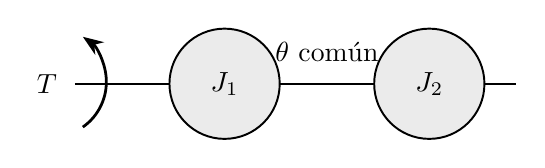
\begin{tikzpicture}[>={Stealth[length=2.6mm]}, line width=0.7pt]
  % eje rigido
  \draw (-3.2,0) -- (2.4,0);
  % torque de entrada
  \draw[->, line width=1pt] (-3.1,-0.55) arc (-55:55:0.7);
  \node[left] at (-3.3,0.0) {$T$};
  % inercias
  \draw[fill=black!8] (-1.3,0) circle (0.7); \node at (-1.3,0) {$J_1$};
  \draw[fill=black!8] (1.3,0) circle (0.7);  \node at (1.3,0) {$J_2$};
  % mismo angulo
  \node[above] at (0,0.15) {$\theta$ común};
\end{tikzpicture}
\end{document}
